\documentclass[usenames,dvipsnames]{beamer}
\usetheme{Copenhagen}
\useinnertheme{circles}
\useoutertheme{split}
\setbeamertemplate{itemize items}[triangle]
\beamertemplatenavigationsymbolsempty

\usepackage[english]{babel}
\usepackage[utf8]{inputenc}
\usepackage[T1]{fontenc}
\usepackage{lmodern}
\usepackage{textcomp}
\usepackage{tikz}
\usepackage{eso-pic}
\usepackage{amsmath}
\usepackage{bookmark}
\usepackage{ifthen}
\usepackage{booktabs}
\usepackage{array}
\usepackage{multirow}
\usepackage{multicol}
\usepackage{fontawesome}
\usepackage{graphicx}
\usepackage{hyperref}
\usepackage{listings}
\usepackage{fancyvrb}
\usepackage{ulem}
\usepackage{xcolor}
%\usepackage{pgfpages}

\usetikzlibrary{calc}
\usetikzlibrary{fit}

\definecolor{logogreen1}{RGB}{52,166,77}
\definecolor{logogreen2}{RGB}{73,180,58}
\definecolor{logogreen3}{RGB}{117,200,44}
\definecolor{logogreen4}{RGB}{157,212,31}
\definecolor{logogreen5}{RGB}{67,149,55}
\definecolor{logogreen6}{RGB}{35,144,63}
\definecolor{titlegreen}{RGB}{72,147,65}
\definecolor{textgrey}{RGB}{138,140,142}
\definecolor{bulletsgreen}{RGB}{171,208,55}

\definecolor{pblue}{rgb}{0.13,0.13,1}
\definecolor{pgreen}{rgb}{0,0.5,0}
\definecolor{pred}{rgb}{0.9,0,0}
\definecolor{pgrey}{rgb}{0.46,0.45,0.48}
\definecolor{pbrown}{RGB}{128,128,0}

\setbeamercolor*{structure}{fg=bulletsgreen}
\setbeamercolor*{palette primary}{fg=white,bg=logogreen3}
\setbeamercolor*{palette quaternary}{fg=white,bg=logogreen6}
\setbeamercolor*{normal text}{fg=textgrey, bg=white}
\setbeamercolor*{titlelike}{fg=titlegreen, bg=white}
\setbeamercolor*{block title}{fg=white, bg=logogreen1}

\makeatletter
\renewcommand{\@makefnmark}{\hbox{\textsuperscript{\tiny{\@thefnmark}}}}
\makeatother

\newenvironment<>{mydef}[1]{%
  \setbeamercolor{block title}{fg=white,bg=logogreen6}%
  \begin{block}#2{#1}}
{\end{block}}

\newenvironment<>{operations}
	{\begin{block}{Operations}{#1}}
	{\end{block}}


\setcounter{tocdepth}{4}
\newboolean{subsectiontoc}
\setboolean{subsectiontoc}{true}
\setbeamerfont{subsubsection in toc}{size=\tiny}
\setbeamertemplate{subsubsection in toc}{\leavevmode\leftskip=3em\inserttocsubsubsection\par}
%\addtobeamertemplate{footline}{\hfill\insertframenumber/\inserttotalframenumber\newline}{}

\AtBeginSection[]
{
  \begin{frame}
  \frametitle{Outline}
  \tiny{\tableofcontents[currentsection,subsubsectionstyle=hide]}
  \end{frame}
}
\AtBeginSubsection[]
{
	\ifthenelse{\boolean{subsectiontoc}}{
		\begin{frame}
			\frametitle{Outline}
			\tiny{\tableofcontents[sectionstyle=show/shaded,currentsubsection,subsubsectionstyle=hide]}
		\end{frame}
	}{
		\begin{frame}
			\frametitle{Outline}
			\tiny{\tableofcontents[sectionstyle=show/shaded,currentsubsection,subsubsectionstyle=show]}
		\end{frame}
	}
}

\newcommand{\deeptocsubsection}[1]{
  \setboolean{subsectiontoc}{false}
  \subsection{#1}
  \setboolean{subsectiontoc}{true}
}

\newcommand\AtPagemyUpperLeft[1]{\AtPageLowerLeft{%
\put(\LenToUnit{0mm},\LenToUnit{3.38mm}){#1}}}%
\AddToShipoutPictureFG{%
  \AtPagemyUpperLeft{{
\includegraphics[width=.5cm,keepaspectratio]{r.png}}}
}

\newcolumntype{C}[1]{>{\centering\let\newline\\\arraybackslash\hspace{0pt}}m{#1}}
\newcolumntype{L}[1]{>{\raggedright\let\newline\\\arraybackslash\hspace{0pt}}m{#1}}
\newlength{\myl}
\newlength{\myll}
\renewcommand{\arraystretch}{1.3}

\makeatletter
\newcommand\colorwave[1][red]{\bgroup \markoverwith{\lower3.5\p@\hbox{\sixly \textcolor{#1}{\char58}}}\ULon}
\font\sixly=lasy6 % does not re-load if already loaded, so no memory problem.
\makeatother

\lstset{
	language=Java,
  commentstyle=\color{pgrey},
  keywordstyle=\color{pblue},
  stringstyle=\color{pgreen},
	frame=tblr
	backgroundcolor=\color{logogreen6},
	extendedchars=true,
	showstringspaces=false,
	showspaces=false,
	tabsize=2,
	breaklines=true,
	showtabs=false,
	captionpos=b,
	basicstyle=\ttfamily\scriptsize\color{black},
	basewidth=0.5em,
	escapechar=\%,
  moredelim=[il][\textcolor{pbrown}]{$$}
}

\makeatletter
\newenvironment{SmallListing}[1][]
  {\lstset{#1}\VerbatimEnvironment\begin{VerbatimOut}{VerbEnv.tmp}}
  {\end{VerbatimOut}\settowidth\@tempdima{%
    \lstinputlisting{VerbEnv.tmp}}
  \minipage{\@tempdima}\lstinputlisting{VerbEnv.tmp}\endminipage}    
\makeatother

\title[{\makebox[.45\paperwidth]{Nieuwigheden in Java 8\hfill}}]{Nieuwigheden Java 8}
\author[{\makebox[.45\paperwidth]{\hfill Maarten Dhondt}}]{Maarten Dhondt}
\institute{Realdolmen}
\date{October 25, 2018}

%\setbeameroption{show notes on second screen=right}

\begin{document}

\frame{\titlepage}

{
\usebackgroundtemplate{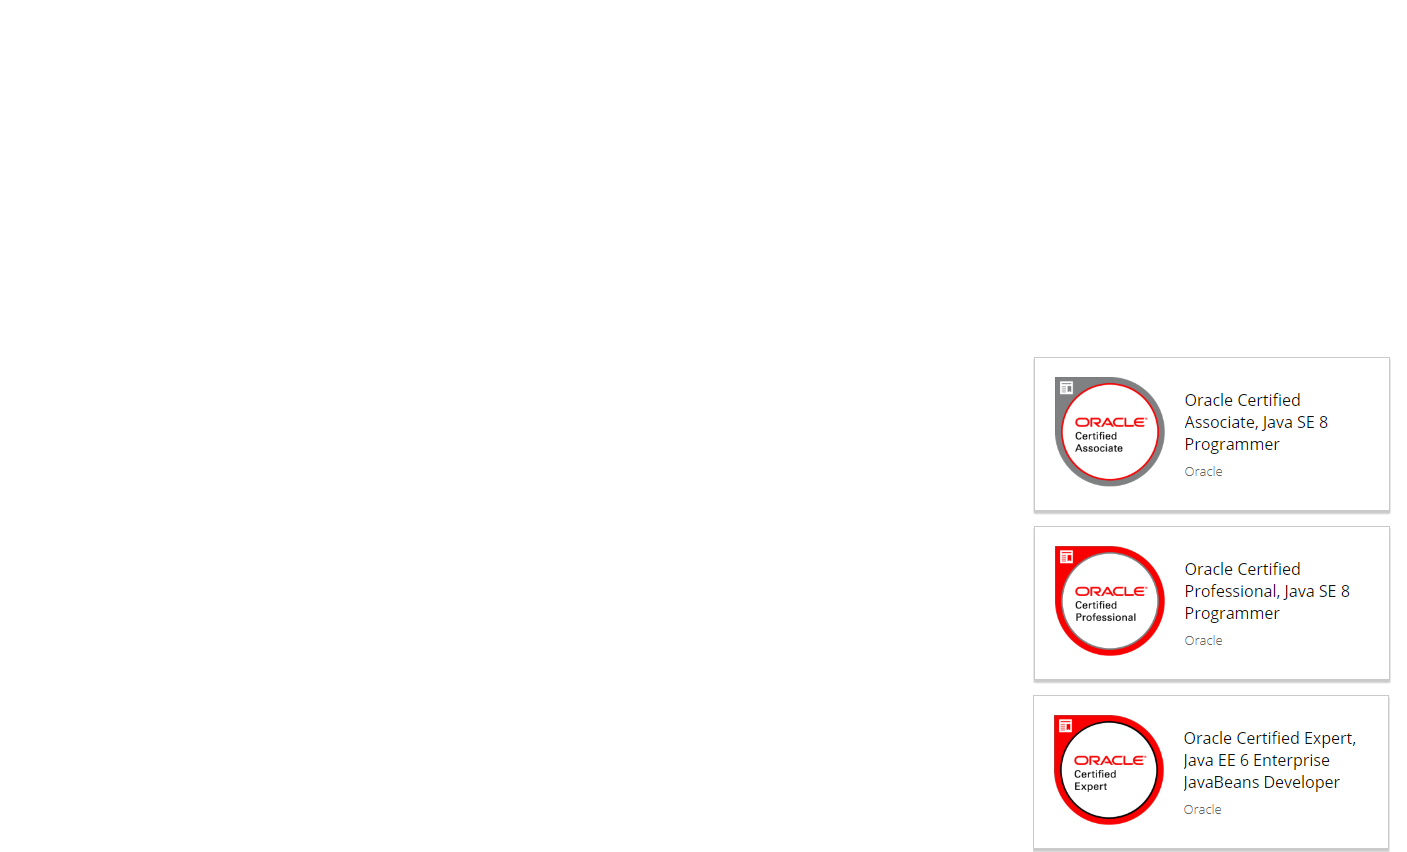
\includegraphics[width=\paperwidth]{badges}}
\begin{frame}
	\frametitle{Wie ben ik?}
	\begin{itemize}\setlength\itemsep{5mm}
		\item Master in de ingenieurswetenschappen: computerwetenschappen (KUL)
		\begin{itemize}
			\item Computationele informatica
		\end{itemize}
		\item Software engineer @ Realdolmen sinds 2015
		\item Projecten: 
		\begin{itemize}
			\item Infrastructuur planning @ Infrabel
			\item API platform @ Proximus
		\end{itemize}
		\item Contact:
		\begin{itemize}
			\item \scalebox{.85}{\faEnvelope}~\href{mailto:maarten.dhondt@realdolmen.com}{maarten.dhondt@realdolmen.com}
			\item \faLinkedinSquare~\href{https://www.linkedin.com/in/maartendhondt/}{maartendhondt}
			\item \faGithubSquare~\href{https://github.com/MDhondt/}{MDhondt}
		\end{itemize}
	\end{itemize}
\end{frame}
}

\title[{\makebox[.45\paperwidth]{Nieuwigheden in Java 8\hfill\insertframenumber/\inserttotalframenumber}}]{Nieuwigheden in Java 8}
\author[{\makebox[.45\paperwidth]{https://github.com/MDhondt/java8-presentation}}]{Maarten Dhondt}

\begin{frame}
  \frametitle{Outline}
  \tiny{\tableofcontents}
\end{frame}

\author{Maarten Dhondt}

\section{Java 8}

\subsection{Interfaces}

\begin{frame}
	\frametitle{Interfaces}
	
	\begin{itemize}
		\item Een interface gelijkt op een klasse, maar bevat enkel methoden en attributen. Interfaces hebben geen geïmplementeerde methoden, maar enkel de signatuur.
		\begin{itemize}
			\item Implementaties hebben dezelfde signatuur maar return type kan een subklasse zijn.
			\item Implementaties gooien geen andere checked exceptions dan diegene uit de interface.
			\item Abstracte klassen kunnen methoden implementeren, maar niet vereist.
		\end{itemize}
	\end{itemize}
\end{frame}

\begin{frame}[fragile]
	\frametitle{Interfaces}
	Implementatie zelfde signatuur maar return type kan subklasse zijn.
	\begin{lstlisting}
public abstract class Transaction {}
	\end{lstlisting}
	\begin{lstlisting}
public class BankTransaction extends Transaction {}
	\end{lstlisting}
	\hrule\vspace{.2cm}
	\begin{lstlisting}
public interface Transactionable {
    Transaction doTransaction();
}
	\end{lstlisting}
	\begin{lstlisting}
public class BankTranserService implements Transactionable {
    @Override
    public BankTransaction doTransaction() {
        ...
    }
}
	\end{lstlisting}
\end{frame}

\begin{frame}[fragile]
	\frametitle{Interfaces}
	Implementatie gooit geen andere checked exceptions.
	\begin{lstlisting}
public interface ExceptionThrowingInterface {
    void doStuff() throws IOException;
}
	\end{lstlisting}
	\begin{lstlisting}
public class ExceptionThrower implements ExceptionThrowingInterface {
    @Override
    public void doStuff() throws IOException, %\colorwave{ReflectionException}% {
				// 'doStuff()' in 'ExceptionThrower' clashes with 'doStuff()' in 'ExceptionThrowingInterface'; overriden method does not throw 'javax.management.ReflectionException'
    }
}
	\end{lstlisting}
\end{frame}

\begin{frame}[fragile]
	\frametitle{Interfaces}
	Abstracte klasse kan methode implementeren, maar niet vereist
	\begin{lstlisting}
public interface Moveable {
    void move();
}
	\end{lstlisting}
	\begin{lstlisting}
public abstract class Furniture implements Moveable {}
	\end{lstlisting}
	\begin{lstlisting}
public class Chair extends Furniture {
    @Override
    public void move() {
        System.out.println("Moved chair");
    }
}
	\end{lstlisting}
\end{frame}

\begin{frame}
	\frametitle{Interfaces}
	\begin{itemize}
		\item Java 8 introduceert \texttt{default} methoden.
		\begin{itemize}
			\item Wat? Een implementatie in de interface.
			\item Waarom? Optionele methoden
			\item Waarom? Gedrag overerving van meerder klassen.
		\end{itemize}
		\item Vorige regels blijven (uiteraard) geldig.
	\end{itemize}
\end{frame}

\begin{frame}[fragile]
	\frametitle{Interfaces}
	\begin{itemize}
		\item Voorbeeld van een \texttt{default} methode.
	\begin{lstlisting}
public interface Animal {

		void eat();
		
		void move();
		
		void sleep();
		
    default void blinkEyes() {
        System.out.println("Blink");
    }
}
	\end{lstlisting}
	\end{itemize}
\end{frame}

\begin{frame}[fragile]
	\frametitle{Interfaces}
	\begin{itemize}
		\item \texttt{default} methoden: optionele methoden.
	\begin{lstlisting}
public interface Collection<E> extends Iterable<E> {

    default boolean removeIf(Predicate<? super E> filter) {
        Objects.requireNonNull(filter);
        boolean removed = false;
        final Iterator<E> each = iterator();
        while (each.hasNext()) {
            if (filter.test(each.next())) {
                each.remove();
                removed = true;
            }
        }
        return removed;
    }
				
}
	\end{lstlisting}
	\end{itemize}
\end{frame}

\begin{frame}
	\frametitle{Interfaces}
	
	Java 8 introduceert ook SAM (Single Abstract Method) interfaces die we functionele interfaces noemen.
	\begin{itemize}
		\item Interface moet exact 1 abstracte methode hebben.
		\item Met of zonder \texttt{@FunctionalInterface} annotatie.
	\end{itemize}
	Kunnen gebruikt worden in lambda expressies en method references
\end{frame}

\begin{frame}[fragile]
	\frametitle{Interfaces}
	
	\begin{lstlisting}
package java.lang;

$$@FunctionalInterface
public interface Runnable {
    public abstract void run();
}
	\end{lstlisting}
	\begin{lstlisting}
public class Main {
    public static void main(String[] args) {
        ExecutorService executor = Executors.newSingleThreadExecutor();
        executor.submit(() -> {
            System.out.println(Thread.currentThread().getName());
        });
    }
}
	\end{lstlisting}
\end{frame}

\subsection{Lambda expressies}

\begin{frame}
	\frametitle{Lambda expressies}
	
	Lambda expressies zijn een nieuwe en belangrijke functie uit Java 8 die:
	\begin{itemize}
		\item op een duidelijke en bondige manier een interface methode beschrijven in een expressie,
		\item een grote verbetering mogelijk maken van de Collection libraries.
	\end{itemize}
\end{frame}

\begin{frame}[fragile]
	\frametitle{Lambda expressies}
	
	\begin{itemize}
		\item Lambda expressies bieden een oplossing aan de verbose anonieme inner klassen door 5 lijnen code te reduceren naar 1 lijn.
		\item Deze horizontale oplossing, lost het verticale probleem van inner klassen op.
		\item Een lambda expressie bestaat uit 3 delen:
		\begin{itemize}
			\item Argumenten lijst
			\item Pijltje: \texttt{->}
			\item Body
		\end{itemize}
	\end{itemize}
	\begin{lstlisting}
(int x, int y) -> x + y
	\end{lstlisting}
\end{frame}

\begin{frame}[fragile]
	\frametitle{Lambda expressies}
	Argumenten lijst:
	\begin{itemize}
		\item Bij slechts 1 argument
	\end{itemize}
\end{frame}

\begin{frame}[fragile]
	\frametitle{Lambda expressies}
	\begin{lstlisting}
public interface LambdaInterface {
  String doStuff(Integer x, String y);
}
	\end{lstlisting}
	\begin{lstlisting}
public class Main {
  public static void main(String[] args) {
    LambdaInterface anonymousImpl = new LambdaInterface() {
      @Override
      public String doStuff(Integer x, String y) {
        return "x=" + x + ",y=" + y;
      }
    };

    LambdaInterface lambdaImpl = (x, y) -> "x=" + x + ",y=" + y;

    System.out.println(anonymousImpl.doStuff(5, "Abc"));
    System.out.println(lambdaImpl.doStuff(5, "Abc"));
  }
}
	\end{lstlisting}
\end{frame}

\subsection{Streams}

\subsection{Java Date / Time API}

\subsection{Overige vernieuwingen}

\subsubsection{Optional}

\subsubsection{StringJoiner}

\subsubsection{Comparators}

\subsubsection{JavaFX}

\subsubsection{Allerlei}

\section{Java 9, 10 \& 11}

\end{document}